The Camera System handles three primary tasks. The motor controller board receives signals from the Processing System. The control board then orients the gimbal to the angles specified by the signals. For the final task, the cameras capture stereo video and pass the video to the Processing System. The Processing System serves as an intermediary between the Camera System and Virtual Reality System. The two functionalities are processing the video and translating the head tracking data. The final system is the Virtual Reality System. This system is responsible for the stereo display of the video and the capture of the raw head tracking data.

\begin{figure}[h!]
	\centering
 	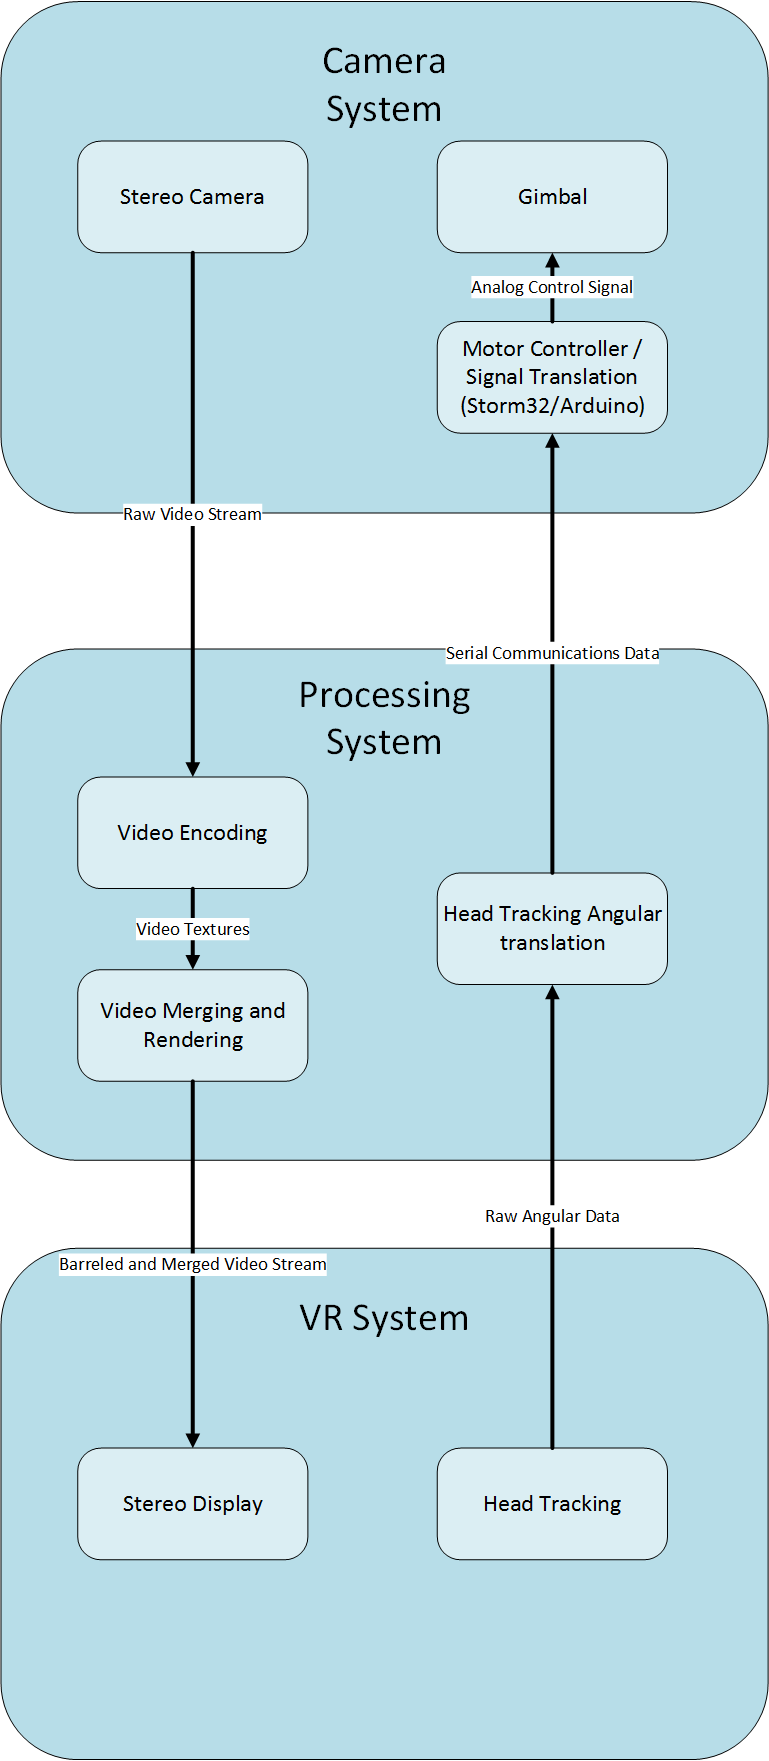
\includegraphics[width=0.27\textwidth]{images/Overview}
 \caption{System architecture}
\end{figure}
